\section{Experimental Evaluation}
\label{sec:evaluation}
To evaluate the \sys{} framework, we
first introduce an experimental setup (\autoref{sec:exp_setup}). Then, we
compare our algorithms against the state of the art for event query
discovery (\autoref{sec:exp_sota}). Finally, we evaluate the sensitivity of
our algorithms with respect to the characteristics of a stream database
(\autoref{sec:exp_sensitity}), before studying the effectiveness of our
strategies to guide the application of discovery algorithms
(\autoref{sec:exp_guidance}).
\subsection{Experimental Setup}
\label{sec:exp_setup}
\sstitle{Datasets}
We leverage both real-world and synthetic data to
evaluate our algorithms.
Specifically, we employ streams of NASDAQ stock trade events~\cite{eodata}
and the Google cluster traces~\cite{reiss2011google}. The
methodology for obtaining stream databases is
adapted from~\cite{ilminer}.
For each dataset, we define three queries to generate streams, as follows.
The event schema for the finance data comprises three attributes: stock
name, volume, and closing value. The queries to construct streams capture
two events with stock name `GOOG' (F1); three events with stock names
appearing in the sequence `AAPL', `GOOG', and `MSFT' (F2); and four events
for which the volume remains constant (F3).
Events in the Google cluster traces contain four attributes:
job ID, machine ID, task status, and priority. One query
defines three events running on the same machine with identical job IDs,
with the first and last ones of status `submit', while the second one has
status `kill' (G1); one query encompasses four events executing on the same
machine with status `finish' (G2); and one query detects job eviction
resulting from the scheduling of another job on the same machine (G3).
Using these queries, we generated the stream databases summarized in
\autoref{tab:databases} by evaluating the queries over the
datasets. For each match (of the first 1000 matches), we constructed a
stream by including the $a$ or
$b=a+1$ events preceding the match. The values of $a$ and $b$, listed in
\autoref{tab:databases}, have been determined experimentally using the
IL-Miner~\cite{ilminer} (described below), i.e., the state of the art for
event query discovery: For a database with streams of length $a$, the
IL-Miner was still
able to compute results, whereas for streams of length $b$, it failed to
compute results within 12 hours. As such, the databases characterize the
computational limit of the state of the art, thereby providing a suitable
basis for the comparison.
Moreover, we employed synthetic data for controlled experiments, which
assess the impact of specific properties of a stream database. For each
evaluation scenario, the dataset was generated by first creating a database
of two streams that do not support any query (i.e., there are neither
supported nor repeated attribute values). Here, the number of events per
stream and the number of attributes may vary for each scenario. Then, the
database is adapted by adding or replacing attribute values, as listed in
\autoref{tab:synt-scenarios}, such that one
database property increases while the others remain constant. The only
exception is that a higher
number of supported attribute values $|\Gamma_D|$ also increases
the {max of sum of supported attribute values}~$\rho_S$.
\begin{table}[t]
	\caption{Stream databases used in the experiments.}
	\label{tab:databases}
	\footnotesize
	\vspace{-1.2em}
	\begin{tabular}{c c c c c }
		\toprule
		\multicolumn{2}{c}{}          & \begin{tabular}[c]{@{}c@{}}stream
			length\\ a | b\end{tabular} & \begin{tabular}[c]{@{}c@{}}number
			of\\
			streams\end{tabular} & \begin{tabular}[c]{@{}c@{}}maximum\\ query
			length\end{tabular} \\
		\midrule
		\multirow{3}{*}{Finance} & F1 & 50 |
		51                                                      &
		79                                                    &
		4                                                              \\
		& F2 & 40 | 41
		& 1000                                                  &
		4                                                              \\
		& F3 & 25 | 26
		& 250                                                   &
		5                                                              \\
		\multirow{1}{*}{Google}  & G1-G3 & 7 |
		8                                                        &
		1000                                                  &
		4                                                              \\
		\bottomrule
	\end{tabular}
	\vspace{-1em}
\end{table}
\begin{table}[t]
	\scriptsize
	\caption{Properties of the synthetic stream databases.}
	\label{tab:synt-scenarios}
	\vspace{-1.2em}
	\begin{tabular}{lcccccc}
		\toprule
		                                          & $|D|$    &
		$|S|$      & $|\mathcal{A}|$ &    $|\Gamma_D|$        &
		$\rho_S$        &   $\rho_R$         \\
		\midrule
		$E_1$                           & \textbf{2,102,...,902} &
		10         & 3          & 0          & 0          & 2          \\
		$E_2$                               & 2          &
		\textbf{6,16,...,96} & 3          & 0          & 0          &
		6          \\
		$E_3$              & 2          & 20         &
		\textbf{1,6,...,101} & 2          & 5          & 5          \\
		$E_4$ & 2          & 102        & 1          &
		\textbf{1,11,...,91} &     $|\Gamma_D|$     & 0          \\
		$E_5$ & 2          & 20         & 3          & 3          &
		\textbf{9,24,...,294} & 6       \\
		$E_6$  & 2          & 20         & 3          & 0          &
		0          & \textbf{2,3,...,13} \\
		\bottomrule
	\end{tabular}
	\vspace{-1.4em}
\end{table}
\sstitle{Baselines}
We compare the algorithms of the \sys{} framework against the
IL-Miner~\cite{ilminer}, the only existing algorithm to discover event
queries with repeated attribute values (see \autoref{sec:related_work}).
Since the IL-Miner, by default, cannot discover queries that comprise query
terms that contain only variables, we consider two variants: one extended
version that can discover these queries, thereby covering the full query
model of the \sys{} framework, and one lossy version that neglects queries
with terms containing no attribute values.
To add another perspective, we include a baseline using a representation
learning algorithm for event streams, as introduced in~\cite{yanli2021}. The
approach learns a probabilistic
automaton to capture events and dependencies that indicate a situation of
interest. While the learned automaton is used for stream monitoring
in~\cite{yanli2021}, a query can be extracted from it by enumerating certain
transition paths~\cite{makowsky2012}. While this
approach
yields only type queries, no pattern queries or mixed queries, a comparison
sheds light on the potential of learning-based techniques for event query
discovery.
\begin{figure*}
	\centering
	\begin{minipage}[c]{0.7\textwidth}
		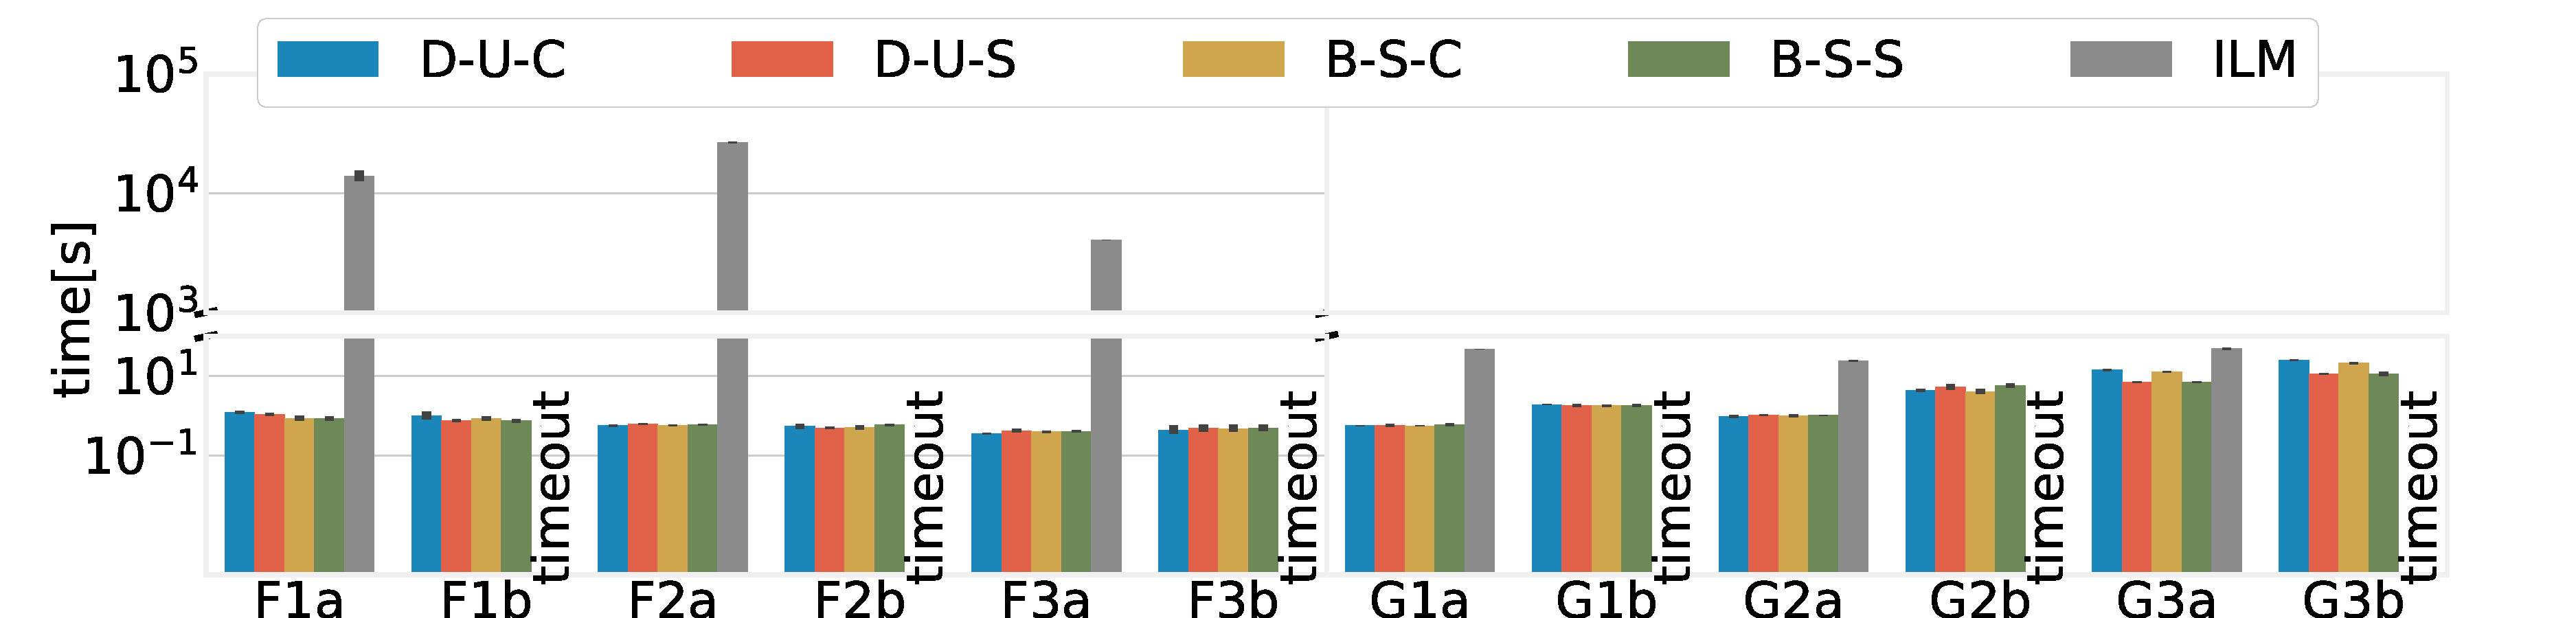
\includegraphics[width=0.95\textwidth]{img/sota_4_broken_new.pdf}
		\vspace{-1em}
		\caption{Runtime comparison with the state of the art.}
	\label{fig:sota}
\end{minipage}
\begin{minipage}[c]{0.29\textwidth}
	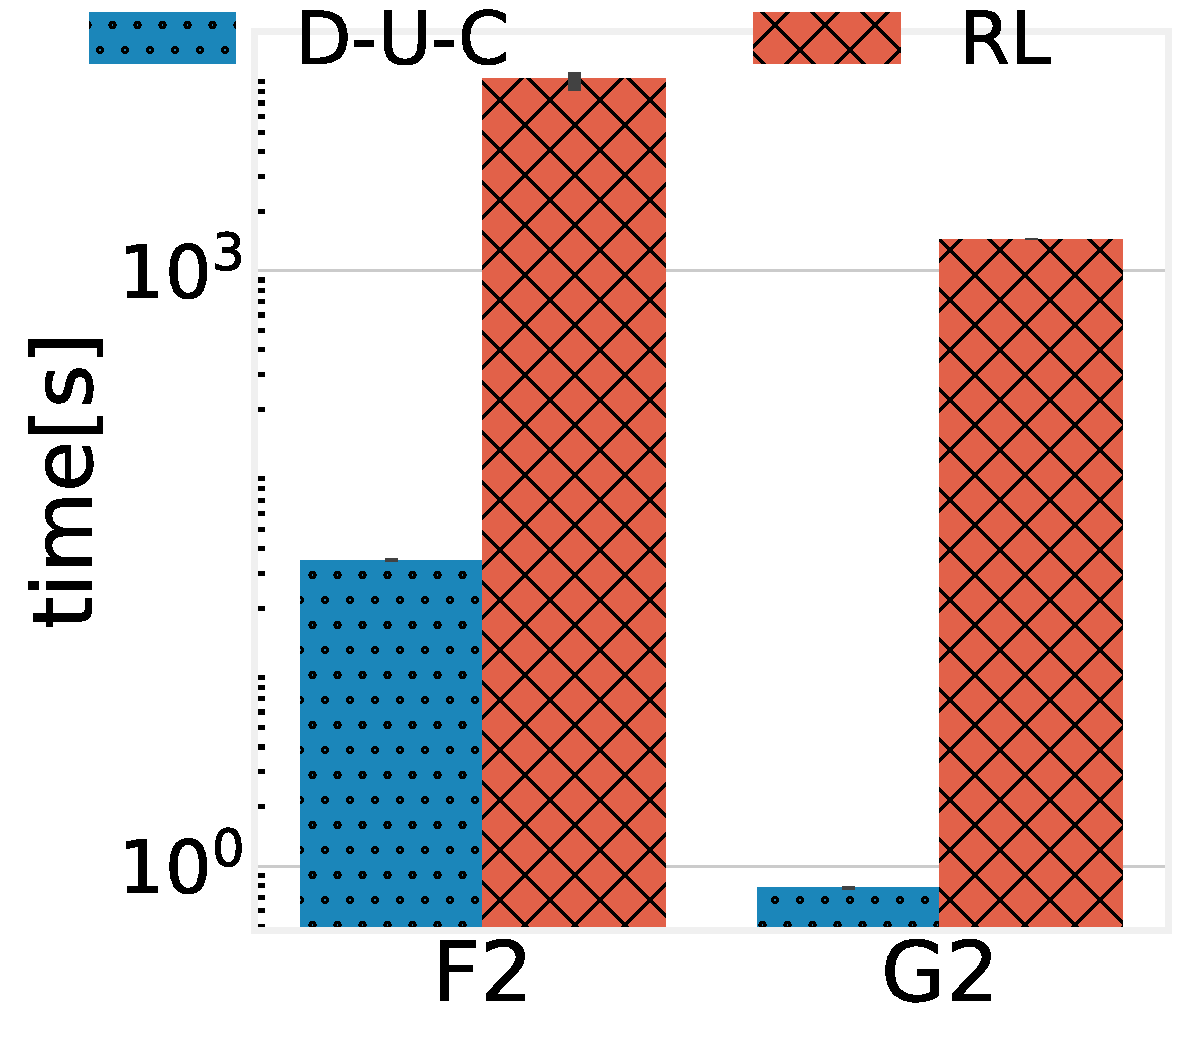
\includegraphics[width=0.65\textwidth]{img/rl_compare.pdf}
	\vspace{-1em}
	\caption{Runtime, RL approach.}
	\label{fig:rl}
\end{minipage}
\vspace{-1em}
\end{figure*}
\sstitle{Measures} We primarily measure the efficiency of event query
discovery in terms of the algorithms' runtime. We report averages over five
experimental runs, including error bars (mostly negligible).
\sstitle{Environment}
We implemented the \sys{} framework in Python. Due to performance issues
of the Java-based version of the IL-Miner and the
absence of a public implementation of the representation learning approach,
we relied on Python-based implementations of the baseline algorithms.
All experiments were conducted on a server with a Xeon 6354 CPU @3,6GHz and
1TB of RAM.
\subsection{State-of-the-Art Comparison}
\label{sec:exp_sota}
First, we compare the runtimes of our algorithms and the
extended IL-Miner, which supports our full query model.
The results in \autoref{fig:sota} show that our algorithms are faster than
the IL-Miner in all cases. For the scenarios based on the finance dataset,
our algorithms are about five orders of magnitude faster. As discussed, we
determined the stream lengths for the $a$ and $b$ scenarios as the
computational limit of the state of the art, i.e., in all $b$ scenarios, the
IL-Miner cannot produce results within 12 hours. The algorithms of the
\sys{} framework enable us to get past this limit in all cases, without a
notable increase in the runtime.
A comparison with the lossy IL-Miner reveals that its improved runtime is traded
for result correctness. The lossy
IL-Miner yields similar runtimes compared to our algorithms, see
\autoref{tab:sota_acc}, yet
it discovers
only a fraction of the queries. That is, with the correct results containing 8
(finance) and 19 (Google) descriptive queries (`Desc'), the lossy IL-Miner
discovers none or only one of them (`Found'), and additionally two and four
queries that are not descriptive (`$\neg$ Desc'). As such, it largely compromises
the result quality not only in terms of descriptiveness, but also in terms of
completeness.
\begin{table}
	\footnotesize
	\caption{Comparison of our algorithms and the lossy IL-Miner.}
	\vspace{-1em}
	\label{tab:sota_acc}
	\begin{tabular}{ c c c c c}
\toprule
Datasets & Avg ${}^{\text{Time Lossy ILM}}/_{\text{Time \sys{}}}$ &
{Desc}(riptive) & Found &
$\neg$
{Desc}\\
\midrule
F1b-F3b & 0.42 & 8 & 0 & 4\\
G1b-G3b & 2.9 & 19 & 1 & 2 \\
\bottomrule
\end{tabular}

	\vspace{-1em}
\end{table}
Finally, we turn to the comparison with the approach based on representation
learning. Since the latter can only discover type queries, we adapted one of our
algorithms (D-U-C) to also return only these queries.
For the datasets F2b and G2b, \autoref{fig:rl} shows the obtained runtime
results, illustrating that our algorithm is at least two orders of magnitude
faster than the baseline algorithm. The effectiveness of query discovery is
summarized in \autoref{tab:rl_compare}. None of the descriptive queries is
discovered by the baseline (`Found'), while only one matching, but not
descriptive query is returned for either scenario (`$\neg$ Desc'). Also, the
construction based on representation learning yields several queries that
are not supported by the stream database (`$\neg$ Matching'). Hence, the
learning-based approach compromises correctness, descriptiveness, and
completeness and, due to high runtimes, is not suitable to address the problem of
event query discovery.
\begin{table}
	\footnotesize
	\caption{Comparison of our algorithms and the RL approach.}
	\vspace{-1em}
	\label{tab:rl_compare}
	\begin{tabular}{ccccc}
\toprule
Dataset & {Desc}(riptive) & Found & $\neg$ {Desc} & $\neg$
Matching\\
\midrule
F2b & 1 & 0 & 1 & 4 \\
G2b & 1 & 0 & 1 & 3 \\
\bottomrule
\end{tabular}

	\vspace{-1em}
\end{table}
\subsection{Sensitivity Analysis}
\label{sec:exp_sensitity}
All of our algorithms show the same worst-case complexity, but incorporate
different design choices. We explore the impact of these choices regarding
properties of stream databases (as introduced in
\autoref{sec:algo_selection}) in a sensitivity analysis.
For the systematically generated stream databases from
\autoref{tab:synt-scenarios}, the results are shown in \autoref{fig:synt_plots}.
Varying the number of streams (E1) leads to generally higher runtimes. As
the size of the database influences the matching of query
candidates, all of our algorithms are effected in the same manner.
An increased length of the streams (E2), as expected (see
\autoref{sec:algo_selection}), has no impact on discovery efficiency. It
does not influence the size of the space of candidate queries to explore.
For the four properties introduced in \autoref{sec:algo_selection} for
algorithm selection, the results
confirm our hypotheses.
\change{A higher number of attributes (E3) favours algorithms that avoid
merging type and pattern queries.
Specifically, D-U-S and D-U-C outperform B-S-S and B-S-C, as merging queries becomes computationally
expensive with more attributes. Increasing the set of
supported attribute values (E4) benefits algorithms that separate the discovery of type and pattern queries.
B-S-S and B-S-C are more efficient under these conditions, due to the
complexity of unified query handling with a large alphabet.
As for the distribution of supported attribute values (E5), D-U-C and B-S-C
perform better due to reduced merge operations.
Conversely, repeated attribute values (E6) favour D-U-S and B-S-S,
as these approaches minimize the search space for pattern queries.}
\change{In sum, our results confirm that the design
choices captured in the \sys{} framework influence the discovery efficiency
as postulated.
The properties of a stream database indeed play a crucial role in
determining which algorithm performs best.}
\begin{figure}
	\centering
	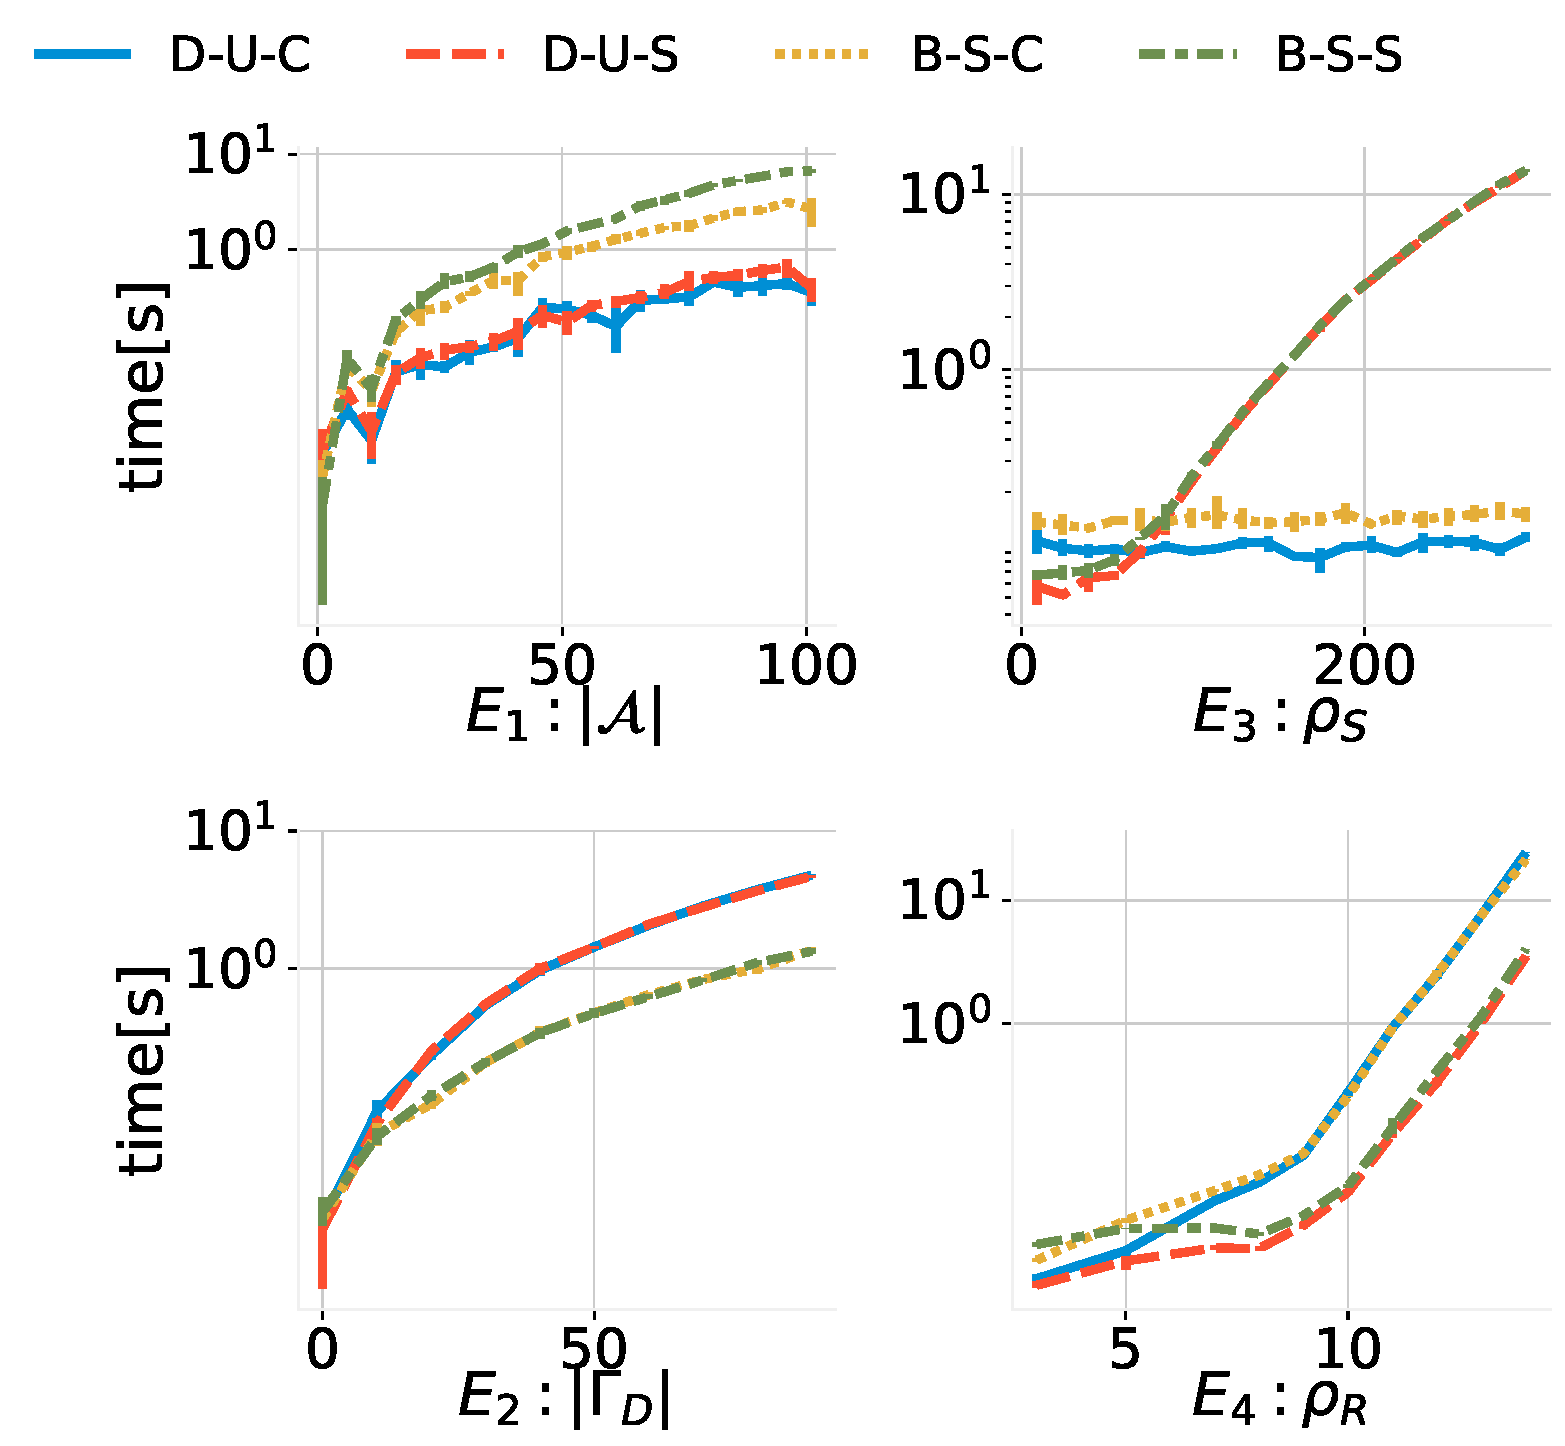
\includegraphics[width=0.95\columnwidth]{img/synt_plots.pdf}
	\vspace{-1em}
	\caption{Sensitivity analysis using synthetic data.}
	\label{fig:synt_plots}
	\vspace{-.5em}
\end{figure}
\subsection{Guidance of Query Discovery}
\label{sec:exp_guidance}
\sstitle{Algorithm selection}
Next, we assess whether the above observations enable us to guide the
selection of a discovery algorithm for the real-world data.
From \autoref{tab:char_corr}, we conclude that the
differences in the number of attributes ($|\mathcal{A}|$) and supported
attribute values ($|\Gamma_D|$) are too small to enable any differentiation,
while the results for the repeated attribute values ($\rho_R$) relate to
an inconclusive value range (see \autoref{fig:synt_plots}). Interestingly,
the measure based on the supported attribute values ($\rho_S$) provides
clues on the runtime performance. For $\rho_S=5$, the algorithms
handling attributes separately (D-U-S and B-S-S) perform much better than
those handling them comprehensively. For $\rho_S>10$, the runtimes of our
algorithms show the opposite trend. Hence, the considered database
properties, assuming that their absolute values provide sufficiently strong
indicators, indeed enable conclusions on the suitability of our algorithms.
\begin{table}[t]
	\footnotesize
	\caption{Correlation of runtime and database properties.}
	\label{tab:char_corr}
	\vspace{-1em}
	\begin{tabular}{cccccccc}
\toprule
\multicolumn{4}{c}{Algorithm Runtime} & \multicolumn{4}{c}{Database
Properties} \\
D-U-C & D-U-S & B-S-C & B-S-S & $\rho_R$ & $\rho_S$ & $|\mathcal{A}|$ & $|\Gamma_D|$ \\
\midrule
18.28 & 26.43 & 17.65 & 26.21 & 6 & 11 & 3 & 2 \\
13.50 & 14.95 & 10.52 & 13.34 & 5 & 17 & 3 & 2 \\
0.65 & 1.39 & 0.88 & 1.68 & 9 & 15 & 3 & 6 \\
259.11 & 364.07 & 226.32 & 366.51 & 10 & 12 & 4 & 1 \\
55.43 & 83.84 & 49.32 & 84.51 & 8 & 10 & 4 & 1 \\
533.90 & 172.54 & 488.45 & 172.37 & 8 & 5 & 4 & 1 \\
\bottomrule
\end{tabular}

	\vspace{-1em}
\end{table}
\sstitle{Feedback mechanisms}
Finally, we tested our mechanisms for feedback on the algorithmic
performance.
First, we assessed whether the exclusion of attribute values may indeed serve
as an abstraction to reduce the discovery runtime.
\autoref{fig:exclude} shows the relative change in
runtimes, when step-wise realizing such an exclusion.
Here, E1 refers to the original database, while for E2-E4, we step-wise
removed the most frequent values of the attribute of the smallest
domain (`volume' for finance, `status' for Google). As expected, the
runtime  decreases. For both datasets, the value
distributions are skewed, so that excluding the most frequent
value (E2) has the largest effect.
Second, we study the abstraction of clustering of attribute values. C1
denotes the original
dataset without clustering. Then, for the Google dataset, we clustered the
`priority' attribute, as adopted in~\cite{reiss2011google} (C2)
and~\cite{reiss2012towards} (C3). For the finance dataset, we clustered the
`close price' into 100 (C2) or 50 (C3)
equally-sized clusters.
\autoref{fig:cluster} highlights that higher numbers of values
within a cluster increase the runtimes. For the finance dataset, the effect
is generally larger and especially affects the algorithms that handle
attributes
comprehensively. However, we
motivated the
abstraction with the desire to increase the result size. For the finance
dataset, we obtain 18 (C1), 30 (C2), and 106 (C3) descriptive queries, while
for the Google dataset, the result includes  202 (C1), 153 (C2), and 298
(C3) queries. We conclude that the expected trend materializes for our data,
even though there is no monotonic relation. The latter is explained
by the fact that clustering may also lead to similar descriptive queries
being merged
into one, which may dominate the effect of having more descriptive queries
due to smaller attribute domains.
\begin{figure}
	\centering
	\begin{minipage}[c]{0.23\textwidth}
		\centering
		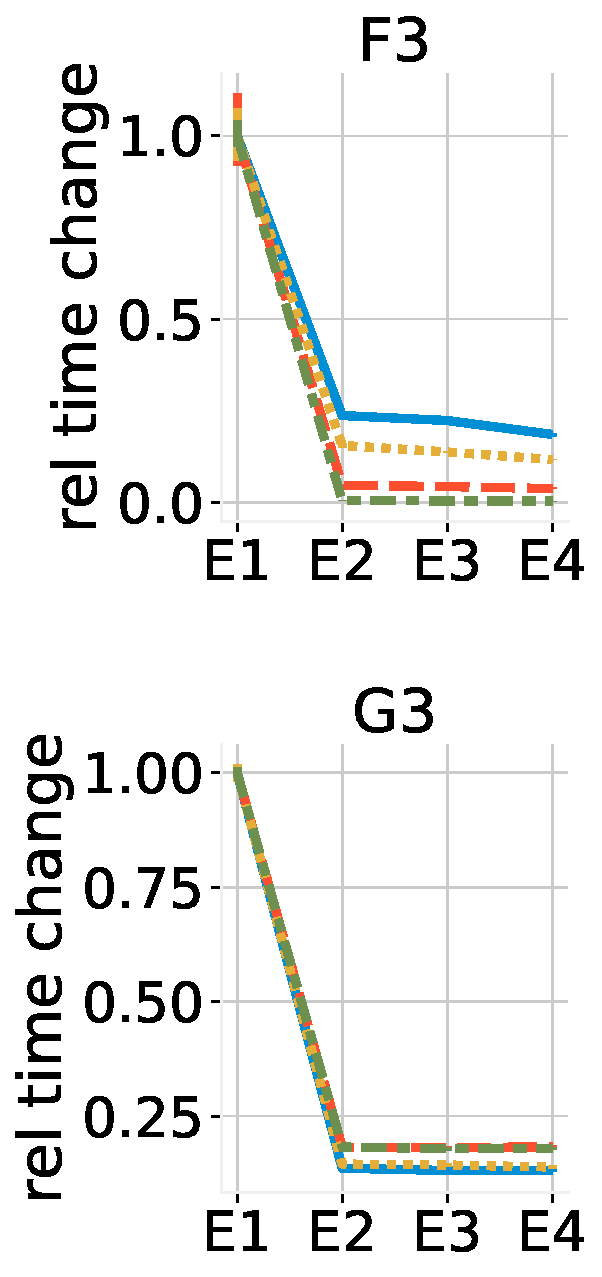
\includegraphics[scale=0.24]{img/exclude.pdf}
		\vspace{-1em}
		\caption{Attr. exclusion.}
		\label{fig:exclude}
	\end{minipage}
	\begin{minipage}[c]{0.23\textwidth}
		\centering
		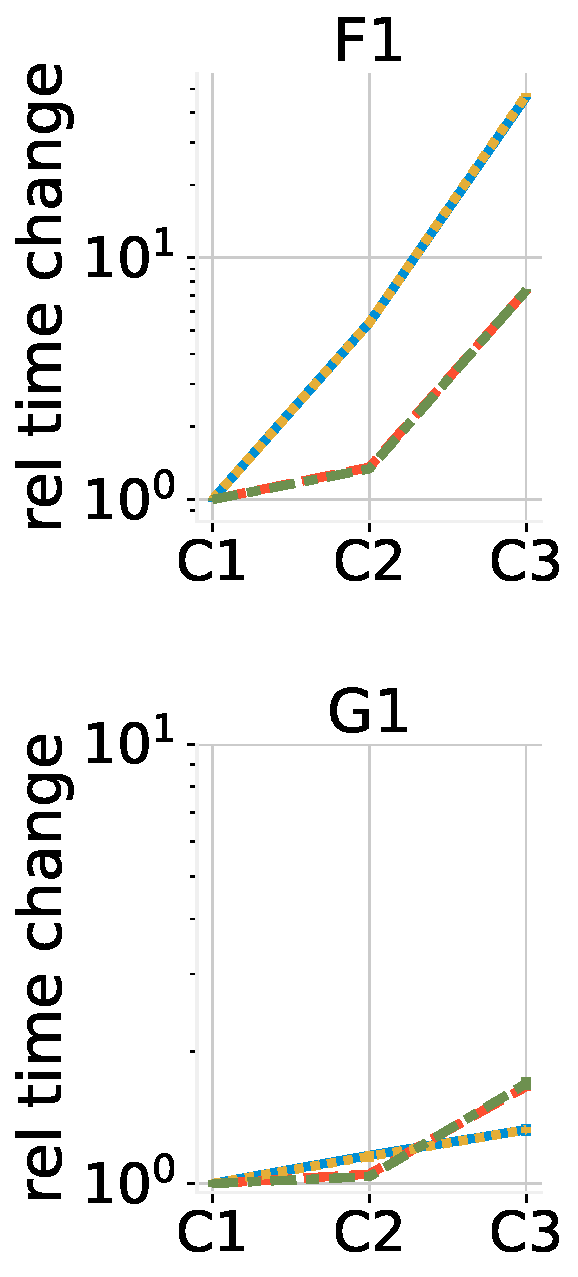
\includegraphics[scale=0.24]{img/cluster.pdf}
		\vspace{-1em}
		\caption{Attr. clustering.}
		\label{fig:cluster}
	\end{minipage}
	\vspace{-1em}
\end{figure}